% interactapasample.tex
% v1.05 - August 2017

\documentclass[]{interact}

\usepackage{booktabs}
\usepackage{longtable}
\usepackage{adjustbox}
\usepackage{amsmath}

%\usepackage[T2A]{fontenc}
%\usepackage[utf8]{inputenc}
%\usepackage[english, russian]{babel}

\usepackage{epstopdf}% To incorporate .eps illustrations using PDFLaTeX, etc.
\usepackage[caption=false]{subfig}% Support for small, `sub' figures and tables
%\usepackage[nolists,tablesfirst]{endfloat}% To `separate' figures and tables from text if required
%\usepackage[doublespacing]{setspace}% To produce a `double spaced' document if required
%\setlength\parindent{24pt}% To increase paragraph indentation when line spacing is doubled

%\usepackage[longnamesfirst,sort]{natbib}% Citation support using natbib.sty
%\bibpunct[, ]{(}{)}{;}{a}{,}{,}% Citation support using natbib.sty
%\renewcommand\bibfont{\fontsize{10}{12}\selectfont}% To set the list of references in 10 point font using natbib.sty
\usepackage[natbibapa,nodoi]{apacite}
\setlength\bibhang{12pt}
\renewcommand\bibliographytypesize{\fontsize{10}{12}\selectfont}

%\usepackage[natbibapa,nodoi]{apacite}% Citation support using apacite.sty. Commands using natbib.sty MUST be deactivated first!
%\setlength\bibhang{12pt}% To set the indentation in the list of references using apacite.sty. Commands using natbib.sty MUST be deactivated first!
%\renewcommand\bibliographytypesize{\fontsize{10}{12}\selectfont}% To set the list of references in 10 point font using apacite.sty. Commands using natbib.sty MUST be deactivated first!

\theoremstyle{plain}% Theorem-like structures provided by amsthm.sty
\newtheorem{theorem}{Theorem}[section]
\newtheorem{lemma}[theorem]{Lemma}
\newtheorem{corollary}[theorem]{Corollary}
\newtheorem{proposition}[theorem]{Proposition}

\theoremstyle{definition}
\newtheorem{definition}[theorem]{Definition}
\newtheorem{example}[theorem]{Example}

\theoremstyle{remark}
\newtheorem{remark}{Remark}
\newtheorem{notation}{Notation}

\begin{document}

%\articletype{ARTICLE TEMPLATE}% Specify the article type or omit as appropriate

%\title{You should call the police: advice from friends and family in victim crime reporting}
\title{Call the cops: advice from friends and family in victim crime reporting}

\author{
	\name{S. Bondarkov\textsuperscript{a}\thanks{CONTACT S. Bondarkov. Email: sbondarkov@eu.spb.ru}}
	\affil{\textsuperscript{a}The Institute for the Rule of Law at the European University at Saint-Petersburg, 6/1~A~Gagarinskaya Street, St.~Petersburg, Russia}
}


\maketitle

\begin{abstract}
TBA
\end{abstract}

\begin{keywords}
Victimization; reporting crime; social support
\end{keywords}

\section{Introduction}

Suppose a rock smashes your window — wrapped around it is a note saying: `You are the gatekeeper of criminal justice system now \citep{gottfredson1987decision}'. That must be confusing. To make sense of what just happened and to figure out a course of action you may want to relate the experience to someone. In the end of this conversation you may choose to mobilize the law by notifiyng the police \citep{black1973mobilization} or to follow the code of the street \citep{anderson1999code%, gangstarr1994code
} and personally confront the frustrated editor that you suspect could not tolerate another opening ``gatekeeper'' citation in a paper on victim reporting behavior\footnote{Whatever you choose, you want to fix that broken window. Or \textit{do} you? \citep{fagan2010street}}.

Victimization is not a light subject, of course, neither are help-seeking or reporting crime to the authorities. The imaginary scenario above is intended not to ridicule, but to fast-forward us past the stage where I am ritually convincing you in precisely that (i.e. in the well established understanding that these are serious problems worth consideration -- which, let's face it, reader, we already agree on) -- and to simultaneously give you the idea of a behavior mechanism that is at the center of this research. 

I assume that, since any victimization is known to be unexpected and cause stress and confusion, if for entirely different reasons, we should expect that a victim of a real crime would also turn to others in order ``to reduce their uncertainty and be reassured'' \citep{ruback1984social}. I argue that, other things being equal, in certain types of crime victimization this decision to seek help in others is the most important factor of reporting the incident to the police. While often overlooked, the importance of social support in victim crime reporting is not unrecognized, as I will show in the next section. However, historically most of the work on the subject was focused on sexualized and intimate partner violence (IPV), evidence for other types of crime remaining scarce \citep{xie2019crime} or, as is the case with cybercrime, non-existent. This is the gap that I address in this paper.

I aim to test whether advice from another person, or, more strictly, the opportunity to talk the incident through with someone a victim relies on, significantly influences the probability that the police will be notified. My perspective on the matter is primarily based on the model of victim decision making developed by Greenberg and Ruback \citep{ruback1984social, ruback_advice_1994, greenberg1992after}: a victim may need help to identify the incident as victimization, in the first place; another person's input -- their emotional support, their perspective on gravity of the accident, on available options of response and on possible consequences -- must also weigh heavy in the decision making process. At the same time, in the spirit of calls for integrative approach \citep{xie2019crime, pescosolido1992beyond}, I attempt to connect social influence model with those suggested in several strains of reporting literature, namely those emphasizing structural factors \citep{black1976behavior}, situational characteristics and (semi-)rational evaluation of those \citep{tarling2010reporting, skogan1984reporting, gottfredson1979study}, attitudes towards criminal justice \citep{goudriaan2004reporting}, and relational distance between offender and victim \citep{felson1999victim}. To this end, I use pooled data from three waves of the Russian Crime Victimization Survey (RCVS) \citep{?} -- a regular and nationally representative monitoring that targets Russian citizens of 18 years and older. 

Traditionally \citep{skogan1976citizen, skogan1984reporting, gottfredson1979study, tarling2010reporting}, gravity of an incident, i.e. perceived actual and potential harm, is seen as the main predictor of reporting to the police. \textit{TBA: add on other frameworks tested by Arina and Kirill.} Recent research by \cite{dzmitryieva2025crime} showed that this view is relevant in Russian context, too. %However, their study was designed to test established reporting theories on a novel set of data -- generated in a cultural context that is different from that in which most of the previous research has taken place. 

\textit{TBA: more findings from Kirill and Arina. More rigorous approach.}

\textit{TBA: Social support framework / world / IPV / some property evidence} However, social support framework, developed mostly in literature on victims of rape and IPV, was left out -- which is all the more natural, given that rape and IPV is out of the scope of RCVS. I build on their result assuming that in other types of crime social support factor is still relevant. I also recognize that post-victimization behavior is known to vary with crime type \citep{?}, so I estimate six separate models on different subsets of data: all violent crime, all property crime, assaults, robberies, thefts, fraud, and, finally, cybercrime.


I find that, after controlling for incident gravity and other possible confounders, the fact of sharing the experience with a confident is the strongest predictor of notifying the police about violent victimization. My modeling suggests that this connection is especially pronounced in cases where the perpetrator is someone close. Turning to property crime, I do not find effect of speaking to others on face-to-face fraud, however, there is a tentative evidence of positive effect of consultation with another person proves on the probability of reporting theft and cybercrime.

My paper contributes to ... 

To my knowledge, this is the first paper to analyze reporting of cybercrime in connection with social support ... 

A by-product of my work is an analysis of personal covariates of seeking help in intimate circle ...

The rest of the paper is conveniently organized the way you would expect. After the literature review in Section \ref{sec:lit_rev}, %the title of which is in view already, 
I will introduce my data (Section \ref{sec:data}) and analytical approach (Section \ref{sec:approach}), present my results (Section \ref{sec:results}), tackle possible effect identification problems (Subsection \ref{subsec:robust}), offer a discussion of findings (Section \ref{sec:discussion}) and conclude with conclusion (Section \ref{sec:conclusion}).

\section{Literature review}
\label{sec:lit_rev}

\subsection{Social support in reporting of crime}

Already the early research on what makes victims delay calling the police found that in most of the cases people first talked to a witness or called someone from the intimate circle before dialing the police \citep{?}.

Psychological literature... Focus on intimate partner violence and sexualized violence...

Bridging the gap: \cite{felstiner1981emergence}, \cite{ruback1984social}, \cite{janoff1986aftermath}, \cite{pescosolido1992beyond}, \cite{greenberg1992after}, 
%Problems are often not simply individual matters. Instead, they frequently represent a shock to a network that calls forth the purpose of or the need for action. 

Later research recognizing the role of counselors: \cite{kaukinen2002help}, \cite{zaykowski2015reconceptualizing}, etc.  

Most recent work, integrative approach: \cite{xie2019crime}, \cite{bergemann2024social}

...which calls for a brief review of main contestants in the field of explaining reporting behavior.

\subsection{Other theoretical frameworks I rely on in this paper}

\paragraph*{Structural} Black and followers.
Motivation for settlement type inclusion: \textit{Black’s (1976) theory has also stimulated research on the social context of victim crime reporting. According to the informal social control model (Black 1976), for example, victims in rural areas are expected to experience more informal social controls and thus are posited to be less likely to report to the police than victims in urban areas (also see Rennison et al. 2013, Ruback \& Menard 2001).}

\paragraph*{Rational choice} Gravity. Limited rationality.

\paragraph*{Attitudes} Towards police. Towards crime. Social context.

\textit{In a review of the evidence for all sides, Baumer (2002) noted that differences in access to informal social controls are inadequate on their own for explaining the variations in victim crime reporting. He proposed a theoretical synthesis, suggesting that victim decisions to notify the police may be influenced not only by access to informal social controls but also more broadly by the availability of alternative nonpolice resources for dealing with crime.}


\section{Data PLACEHOLDER}
\label{sec:data}

\textit{In this analysis, we used pooled cross-sectional data obtained by merging two waves of the Russian Crime Victimization Surveys, conducted in 2018 and 2021 (Knorre, 2019, 2022). These surveys employed nearly identical questionnaires and shared a consistent methodology, which made their integration analytically sound. This approach increases statistical power and the precision of estimates (Verbeek, 2008), with year fixed effects included in the analysis to control for differences between the survey periods. The surveys were conducted using Computer-Assisted personal communication (CATI) with Random Digit Dialing (RDD) of mobile phone numbers. In this approach, the system generates a random number, invites a call, and if a respondent answers, the operator proceeds with the interview.} 

\textit{The survey achieved a 14.1\% completion rate among individuals who answered the phone call. Of the people who answered the phone, 16.5\% agreed to answer the interviewer’s question, and of those who agreed, 85.5\% proceeded to complete the full survey. Although CATI with RDD is not commonly used in victimisation research, this strategy proved more appropriate in the Russian context, where large-scale falsifications by field interviewers in face-to-face surveys are a persistent problem (Rogozin \& Ipatova, 2015). }

\textit{Both surveys implemented a simple random sampling strategy, aiming to interview 3,000 individuals who had experienced victimisation within the past five years. Additionally, participants were also asked about their victimisation experiences in the past twelve months. The survey instruments captured data from both victims and non-victims, collecting detailed information on socio-demographic characteristics, income, and experiences with crime. The survey was conducted across all geographical areas of the country, covering approximately 3,500 locations. }

\textit{Both the RCVS2018 and RCVS2021 surveys achieved a high degree of representativeness at the national level based on key socio-demographic indicators (Serebrennikov \& Titaev, 2022; Verkeev et al., 2019). A comparison of the respondents’ principal sociodemographic characteristics with data from the Federal State Statistics Service of Russia (GKS, 2019) and the Comprehensive Survey of Living Conditions of the Population (KOUZ, 2020) reveals statistically insignificant differences in age and gender. However, the RCVS sample shows a slight skew in age and education level, with those aged 65 and older underrepresented and individuals with higher education overrepresented. This bias can be attributed to the lower availability of the elderly for personal communication due to health or technological barriers, and the higher availability of educated individuals. As is often the case, marginalised populations are less accessible to survey methodologies, potentially leading to missing data on major violent crimes (Verkeev et al., 2019). }

\textit{The questionnaires used in RCVS2018 and RCVS2021 were nearly identical. The RCVS2018 questionnaire was developed through in-depth interviews with victims of various crimes and an extensive review of victimisation surveys in other countries (Verkeev et al., 2019). In early 2021, a methodological audit of the RCVS2018 was conducted, leading to minor revisions and the inclusion of new questions. However, these revisions did not affect the variables used in the present analysis. Since not all events reported to the police meet the legal definition of a crime, this study uses the term “incident” to refer to any such reported event, regardless of its legal qualification. }

\textit{Victims were identified based on their response to the following survey question: “Please recall whether you were robbed, assaulted, threatened, or were a victim of violence, fraud, or other crimes in Russia during the last 5 years?” Respondents who answered affirmatively were classified as victims for this analysis. Table 1 presents descriptive statistics from the two surveys, showing the initial distribution of victims and non-victims. For the purposes of our analysis, only respondents who reported victimisation were included. The data were analysed using the statistical analysis software Stata version 14, and were prepared, cleaned, and captured in the Statistical Package for Social Sciences (SPSS) version 25 prior to analysis.}

TBA:

Add on raking procedure.

Table \ref{table:table1} describes the data I use... It is evident that most people do inform someone close about victimization incident and that it is positively correlated with reporting to the police. However, as I show in Section \ref{sec:approach}, at this point we should rather attribute this to multiple confounders of the two variables...

Table \ref{?} in Appendix documents questions behind the variables and my aggregation decisions...

\begin{table}[p]
	\caption{Victimization and reported incidents share tabulated by variables used in this study}
	\label{table:table1}
	\begin{adjustbox}{width=1\textwidth, height=4in}
		\begin{tabular}{p{1.2in}p{1.2in}rrrrrrrrrr}
	\toprule
	&  & \multicolumn{2}{c}{Cybercrime    } & \multicolumn{2}{c}{Fraud    } & \multicolumn{2}{c}{Theft    } & \multicolumn{2}{c}{Assault    } & \multicolumn{2}{c}{Robbery    } \\ 
	\cmidrule(lr){3-4} \cmidrule(lr){5-6} \cmidrule(lr){7-8} \cmidrule(lr){9-10} \cmidrule(lr){11-12}
	&     & N & Rep. (SE) & N  & Rep. (SE)  & N   & Rep. (SE)   & N    & Rep. (SE)    & N     & Rep. (SE)     \\ 
\vspace{1.5pt}\\
 & Total & 2074 & 0.47 (0.01) & 600 & 0.45 (0.02) & 1893 & 0.61 (0.01) & 790 & 0.56 (0.02) & 340 & 0.67 (0.03) \\ 
 Year & 2018 & 474 & 0.45 (0.02) & 351 & 0.39 (0.03) & 905 & 0.61 (0.02) & 229 & 0.53 (0.03) & 150 & 0.71 (0.04) \\ 
 & 2021 & 865 & 0.45 (0.02) & 214 & 0.53 (0.03) & 562 & 0.63 (0.02) & 276 & 0.59 (0.03) & 104 & 0.69 (0.05) \\ 
 & 2024 & 735 & 0.51 (0.02) & 35 & 0.73 (0.08) & 426 & 0.59 (0.02) & 285 & 0.56 (0.03) & 86 & 0.6 (0.05) \\
	\vspace{1pt}\\
%	\midrule
	\multicolumn{12}{l}{\textsc{Panel A. Socioeconomic status}} \\
		% \addlinespace[4pt]
Gender & Female & 1129 & 0.48 (0.01) & 294 & 0.48 (0.03) & 938 & 0.63 (0.02) & 299 & 0.62 (0.03) & 129 & 0.77 (0.04) \\ 
 & Male & 945 & 0.46 (0.02) & 306 & 0.42 (0.03) & 955 & 0.6 (0.02) & 491 & 0.52 (0.02) & 211 & 0.61 (0.03) \\ 
	%	% \addlinespace[4pt]
	\midrule
Age & 18-24 & 193 & 0.33 (0.03) & 39 & 0.49 (0.08) & 165 & 0.37 (0.04) & 134 & 0.35 (0.04) & 52 & 0.41 (0.07) \\ 
 & 25-34 & 513 & 0.44 (0.02) & 138 & 0.31 (0.04) & 454 & 0.63 (0.02) & 218 & 0.49 (0.03) & 88 & 0.55 (0.05) \\ 
 & 35-49 & 756 & 0.49 (0.02) & 195 & 0.49 (0.04) & 654 & 0.67 (0.02) & 282 & 0.64 (0.03) & 119 & 0.66 (0.04) \\ 
 & 50-64 & 414 & 0.48 (0.02) & 137 & 0.55 (0.04) & 411 & 0.56 (0.02) & 120 & 0.7 (0.04) & 57 & 0.86 (0.05) \\ 
 & 65+ & 198 & 0.59 (0.04) & 91 & 0.4 (0.05) & 207 & 0.7 (0.03) & 36 & 0.84 (0.06) & 23 & 0.94 (0.05) \\ 

	\midrule
Has partner & No & 790 & 0.47 (0.02) & 249 & 0.45 (0.03) & 694 & 0.57 (0.02) & 383 & 0.52 (0.03) & 143 & 0.65 (0.04) \\ 
 & Yes & 1284 & 0.47 (0.01) & 351 & 0.45 (0.03) & 1199 & 0.64 (0.01) & 407 & 0.6 (0.02) & 197 & 0.69 (0.03) \\ 

	\midrule
Settlement type & City & 1415 & 0.48 (0.01) & 438 & 0.45 (0.02) & 1291 & 0.62 (0.01) & 536 & 0.52 (0.02) & 235 & 0.63 (0.03) \\ 
 & Small town & 306 & 0.45 (0.03) & 88 & 0.46 (0.05) & 313 & 0.6 (0.03) & 116 & 0.59 (0.05) & 50 & 0.84 (0.05) \\ 
 & Village & 303 & 0.47 (0.03) & 57 & 0.45 (0.07) & 227 & 0.61 (0.03) & 111 & 0.7 (0.04) & 48 & 0.76 (0.06) \\ 
 & Unknown & 50 & 0.39 (0.07) & 17 & 0.4 (0.12) & 62 & 0.65 (0.06) & 27 & 0.65 (0.09) & 7 & 0.51 (0.21) \\ 

	\midrule
Education & School & 250 & 0.49 (0.03) & 100 & 0.31 (0.05) & 266 & 0.55 (0.03) & 177 & 0.5 (0.04) & 65 & 0.65 (0.06) \\ 
 & Vocational & 661 & 0.47 (0.02) & 214 & 0.5 (0.03) & 645 & 0.62 (0.02) & 298 & 0.57 (0.03) & 108 & 0.69 (0.04) \\ 
 & Tertiary & 1159 & 0.47 (0.01) & 286 & 0.48 (0.03) & 981 & 0.64 (0.02) & 311 & 0.62 (0.03) & 166 & 0.7 (0.04) \\ 

    \midrule
Employment & Unemployed & 298 & 0.5 (0.03) & 82 & 0.69 (0.05) & 269 & 0.53 (0.03) & 146 & 0.62 (0.04) & 54 & 0.61 (0.07) \\ 
 & Pensioner & 352 & 0.54 (0.03) & 151 & 0.41 (0.04) & 362 & 0.67 (0.02) & 80 & 0.79 (0.05) & 44 & 0.9 (0.05) \\ 
 & Worker & 369 & 0.43 (0.03) & 105 & 0.39 (0.05) & 365 & 0.55 (0.03) & 197 & 0.51 (0.04) & 73 & 0.63 (0.06) \\ 
 & Manager & 417 & 0.41 (0.02) & 119 & 0.34 (0.04) & 370 & 0.67 (0.02) & 137 & 0.56 (0.04) & 75 & 0.62 (0.06) \\ 
 & Employee & 451 & 0.5 (0.02) & 94 & 0.5 (0.05) & 348 & 0.63 (0.03) & 119 & 0.61 (0.05) & 51 & 0.71 (0.06) \\ 
 & Student & 187 & 0.38 (0.04) & 49 & 0.51 (0.07) & 179 & 0.55 (0.04) & 111 & 0.36 (0.05) & 43 & 0.47 (0.08) \\ 



	%	% \addlinespace[4pt]
	\midrule
	Income level & Low%Can afford buying clothes, or lower 
    & 456 & 0.54 (0.02) & 24 & 0.86 (0.07) & 265 & 0.61 (0.03) & 180 & 0.58 (0.04) & 59 & 0.71 (0.06) \\ 
	& Middle%Can afford buying furniture and electronics 
    & 203 & 0.5 (0.04) & 7 & 0.68 (0.19) & 107 & 0.63 (0.05) & 61 & 0.67 (0.06) & 15 & 0.59 (0.13) \\ 
	& High%Can afford buying a car, or higher 
    & 58 & 0.42 (0.07) & 4 & 0.14 (0.18) & 39 & 0.57 (0.08) & 34 & 0.34 (0.08) & 6 & 0.23 (0.19) \\ 
%	\midrule
		\vspace{1pt}\\
		\multicolumn{12}{l}{\textsc{Panel B. Incident characteristics}} \\
	% \addlinespace[4pt]
	Damage: money, %thnd rubles 
    & [0,1] & 263 & 0.21 (0.03) & 70 & 0.21 (0.05) & 249 & 0.5 (0.03) & 599 & 0.53 (0.02) & 49 & 0.58 (0.07) \\ 
thnd rubles  & (1,10] & 825 & 0.36 (0.02) & 159 & 0.27 (0.04) & 592 & 0.5 (0.02) & 81 & 0.63 (0.05) & 105 & 0.64 (0.05) \\ 
 & (10,50] & 523 & 0.51 (0.02) & 145 & 0.51 (0.04) & 647 & 0.65 (0.02) & 53 & 0.6 (0.07) & 111 & 0.71 (0.04) \\ 
 & (50,Inf] & 463 & 0.74 (0.02) & 226 & 0.65 (0.03) & 405 & 0.79 (0.02) & 57 & 0.82 (0.05) & 75 & 0.73 (0.05) \\
	\midrule
	Damage: physical & No & &  & &  & &  & 137 & 0.42 (0.04) & 42 & 0.66 (0.07) \\ 
 & Light & &  & &  & &  & 381 & 0.53 (0.03) & 130 & 0.66 (0.04) \\ 
  & Heavy & &  & &  & &  & 272 & 0.69 (0.03) & 90 & 0.7 (0.05) \\ 
\midrule
	% Damage: emotional & Light & 55 & 0.32 (0.06) & &  & 31 & 0.39 (0.09) & 35 & 0.37 (0.08) & 2 & 0 (0) \\ 
	% & Medium & 180 & 0.34 (0.04) & 8 & 0.25 (0.16) & 115 & 0.58 (0.05) & 70 & 0.4 (0.06) & 17 & 0.36 (0.12) \\ 
	% & Heavy & 493 & 0.59 (0.02) & 27 & 0.89 (0.06) & 273 & 0.64 (0.03) & 180 & 0.64 (0.04) & 67 & 0.73 (0.05) \\ 
	% 	\midrule
Incident: there% was a witness 
& No & 1177 & 0.45 (0.01) & 218 & 0.4 (0.03) & 1050 & 0.66 (0.01) & 299 & 0.53 (0.03) & 156 & 0.66 (0.04) \\ 
was a witness  & Yes & 897 & 0.5 (0.02) & 382 & 0.48 (0.03) & 843 & 0.56 (0.02) & 491 & 0.58 (0.02) & 184 & 0.69 (0.03) \\ 
 \midrule
Incident: offender %had a weapon 
& No &  &  &  &  &  &  & 544 & 0.53 (0.02) & 175 & 0.67 (0.04) \\ 
had a weapon  & Yes &  &  &  &  &  &  & 246 & 0.64 (0.03) & 89 & 0.68 (0.05) \\ 
 \midrule
Incident: resisted & No/Doubt &  &  &  &  &  &  & 220 & 0.69 (0.03) & 101 & 0.73 (0.04) \\ 
 & Yes &  &  &  &  &  &  & 570 & 0.51 (0.02) & 163 & 0.63 (0.04) \\
%	\midrule
	\vspace{1pt}\\
		\multicolumn{12}{l}{\textsc{Panel C. Social factors}} \\
	% \addlinespace[4pt]
Offender-victim %relationship 
& Stranger & 1047 & 0.5 (0.02) & 409 & 0.43 (0.02) & 56 & 0.5 (0.07) & 450 & 0.51 (0.02) & 189 & 0.62 (0.04) \\ 
relationship  & Acquaintance & 38 & 0.68 (0.08) & 75 & 0.51 (0.06) & 12 & 0.64 (0.14) & 84 & 0.53 (0.05) & 32 & 0.65 (0.09) \\ 
 & Colleague & 12 & 0.81 (0.12) & 59 & 0.34 (0.06) & 4 & 0.6 (0.29) & 18 & 0.89 (0.08) & 9 & 0.58 (0.18) \\ 
 & Neighbor & 4 & 0.85 (0.19) & 13 & 0.88 (0.1) & 3 & 0.69 (0.33) & 61 & 0.91 (0.04) & 15 & 1 (0) \\ 
  & Friend or relative & 13 & 0.62 (0.14) & 35 & 0.67 (0.08) & 3 & 0.51 (0.35) & 59 & 0.57 (0.06) & 16 & 0.93 (0.07) \\ 
 & Spouse or partner & 5 & 0.55 (0.25) & 2 & 0.71 (0.45) & 2 & 0 (0) & 50 & 0.57 (0.07) & 20 & 0.83 (0.09) \\ 
 \midrule
Victim informed %friends or relatives 
& No & 321 & 0.37 (0.03) & 62 & 0.28 (0.06) & 137 & 0.46 (0.04) & 144 & 0.21 (0.03) & 46 & 0.45 (0.07) \\ 
friends or relatives  & Yes & 1753 & 0.49 (0.01) & 538 & 0.47 (0.02) & 1756 & 0.63 (0.01) & 646 & 0.65 (0.02) & 294 & 0.71 (0.03) \\
	\vspace{1pt}\\
		\multicolumn{12}{l}{\textsc{Panel D. Attitude towards police}} \\
	% \addlinespace[4pt]
Knows a police & No & 1044 & 0.49 (0.02) & 306 & 0.46 (0.03) & 918 & 0.62 (0.02) & 349 & 0.57 (0.03) & 168 & 0.68 (0.04) \\ 
 & Yes & 1026 & 0.45 (0.02) & 294 & 0.45 (0.03) & 975 & 0.6 (0.02) & 439 & 0.56 (0.02) & 170 & 0.69 (0.04) \\ 
Has crime record & No & 1914 & 0.47 (0.01) & 550 & 0.45 (0.02) & 1751 & 0.61 (0.01) & 646 & 0.57 (0.02) & 266 & 0.67 (0.03) \\ 
 & Yes & 159 & 0.46 (0.04) & 50 & 0.47 (0.07) & 141 & 0.67 (0.04) & 142 & 0.52 (0.04) & 73 & 0.73 (0.05) \\ 

	\bottomrule
	\vspace{1pt}\\
	\multicolumn{12}{l}{\small Proportions of reported victimizations and standard errors were calculated with weights obtained in raking procedure.}
\end{tabular}
	\end{adjustbox}
\end{table}

\section{Analytical approach}
\label{sec:approach}

\begin{figure}
	\centering
	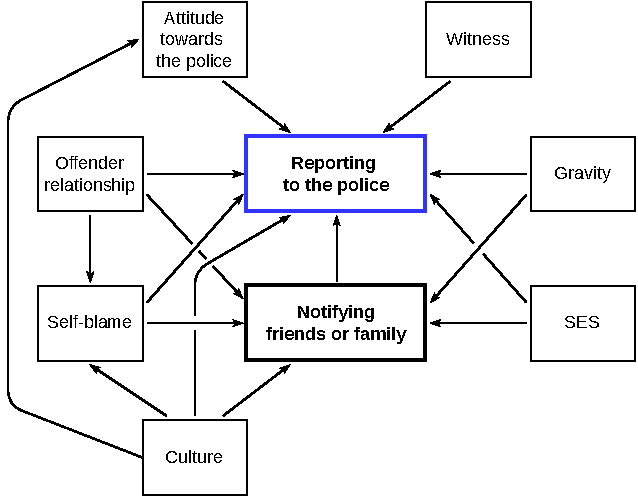
\includegraphics[width = .7\textwidth]{figures/causal_diagram_1.pdf}
	\caption{Causal diagram of decision making model}
	\label{fig:causal_diagram}	
\end{figure}

\subsection{Dependent variable} 
Definition of reporting, definitions of crime types (wording in questionaire).

\subsection{Independent variables} 
A visual summary of causal relations in my model provided in Fig \ref{fig:causal_diagram} makes it evident that an integrative framework is not merely reasonable or theoretically sound but plain necessary if one aims to identify the effect of social support on reporting. Almost all the factors that are supposed to influence the decision to notify the police may as well influence the decision to seek help in friends and family. In other words, the dependent and the focus independent variables have multiple confounders. This poses a threat to identification, which I am able to overcome by inclusion of a broad range of controls. However, there are three caveats. 

First, I do not observe a victim's cultural context. The only way I am able to try to control for it is to introduce federal district fixed effects and settlement type variable, which is better than nothing but admittedly a very crude solution, because context may vary greatly across a city, not to mention a federal district \citep{goudriaan2006neighbourhood}. 

Second, I do not observe offenders characteristics other than their gender and relation to a victim. I do not include offender gender or interaction of victim-offender genders in my modeling because in my data almost the crime was committed by men. I do include relationship distance which proves to be an important factor. Still, I know nothing of offender's resourcefulness which must be one of the serious considerations in a victim's decision making process. This is an important omission, but one that my study shares with virtually all the research on reporting.

Third, I know only if the police was notified and if a victim told about the incident to someone in their intimate circle -- and I do not know which came first. This means endogeneity is possible: a victim may report to the police and then relate the whole story to friends or family \textit{because} of how the interaction with the police has worked out. While our knowledge of post-victimization behavior suggests that if someone is notified at all then friends or family come before the police \citep{}, the doubt remains. I address this issue in Subsection \ref{subsec:robust} by introducing a supporting model of different design. 

Motivation for year fixed effects:
\textit{Some scholars have attributed substantive meanings to this change and argued that it was caused by changes in sex-role attitudes in the United States (e.g., Orcutt \& Faison 1988) or by the success of rape law reforms and media campaigns (e.g., Bachman 1993, Spohn \& Horney 1992). The evidence from the United Kingdom similarly supported the notion that research and policy attention to rape, sexual assault, and domestic violence had led to more adequate handling of such crimes and that this had resulted in a greater willingness of victims to report crimes by intimate friends and relatives (Tarling \& Morris 2010).}

My main model is logistic regression of the following specification:

\begin{multline}
 \label{eq:1}
    P(Reported_i) =
    g(\beta_1 ToldSomeone_i + \beta_2 Relationship_i \\ + \beta_x SES_i + \beta_y Incident_i + \beta_z Attitude_i + \lambda + \gamma)
\end{multline}
   
where $g(.)$ is logit function, $ToldSomeone$ is an indicator of informing friends or relative, $SES$ is a vector of socioeconomic status variables, $Incident$ -- a vector of situational characteristics, $Attitude$ -- a vector of variables that capture a victim's attitude towards police,  $\lambda$ and $\gamma$ are federal district and year fixed effects.

I run this model on six subsets of victim only data split by crime type: theft, face-to-face fraud, cybercrime, all property crime, assault, all violent crime.

\section{Results}
\label{sec:results}

Regression results in Table \ref{table:regr_pooled} offer both expected and unexpected findings...

It may be more instructive to assess predictions from the model in Fig \ref{fig:predictions}: ...

\begin{table}[htb!]
	\caption{Logistic regression result}
	\label{table:regr_pooled}
	\begin{adjustbox}{width=1\textwidth}
		\begin{tabular}{lcccccc}
\toprule
  & Theft & Fraud & Cybercrime & All property & Assault & All violent \\ 
\midrule\addlinespace[2.5pt]
Told someone & 0.811+ & 1.005 & 0.769 & 0.744+ & 2.100* & 2.152* \\ 
Financial: (1, 10] thnd rub. & 0.138 & 0.612 & 0.929 & 0.440+ & 0.859 & 0.641 \\ 
Financial: (10, 50] thnd rub. & 0.852 & 1.645+ & 1.578 & 1.144* & 0.183 & 0.388 \\ 
Financial: (50, Inf] thnd rub. & 1.477* & 2.178+ & 2.626* & 1.889* & 1.055+ & 1.229+ \\ 
Physical: Light &  &  &  &  & 0.286 & 0.424 \\ 
Physical: Heavy &  &  &  &  & 1.162 & 1.129 \\ 
Incident: Witness &  &  &  &  & 0.373 & 0.276 \\ 
Incident: Victim resisted &  &  &  &  & -0.422 & -0.419 \\ 
Incident: Weapon &  &  &  &  & 0.323 & 0.256 \\ 
Self-blame & -0.620* & -0.163 & -0.614+ & -0.612* & -0.040 & -0.285 \\ 
Has partner & 0.098 & -0.279 & -0.031 & -0.027 & 0.096 & -0.003 \\ 
Off. rel.: Acquaintance or colleague &  &  &  &  & 0.588 & 0.342 \\ 
Off. rel.: Neighbour &  &  &  &  & 1.213 & 1.396 \\ 
Off. rel.: Spouse, partner, relative, friend &  &  &  &  & -0.114 & 0.099 \\ 
Gender: Male & -0.309 & -0.229 & -0.133 & -0.195+ & -0.458 & -0.416 \\ 
Income: Can buy furniture/electonics & -0.015 & 0.273 & 0.170 & 0.113 & 0.085 & -0.002 \\ 
Income: Can buy a car, or higher & 0.203 & 0.350 & -0.435+ & -0.053 & 0.018 & 0.019 \\ 
Highly educated & 0.104 & -0.031 & -0.038 & 0.016 & 0.183 & 0.155 \\ 
Settlement: Small town & -0.175 & 0.408 & -0.116 & -0.050 & 0.974 & 1.040 \\ 
Settlement: Village & -0.123 & -0.281 & -0.096 & -0.108 & 0.476 & 0.429 \\ 
Settlement: Unknown & 0.076 & 0.104 & 0.116 & -0.121 & 0.665 & 0.616 \\ 
Attitude: Victim knows a police & -0.058 & -0.227 & -0.202 & -0.114 & -0.028 & 0.142 \\ 
{Attitude: Victim has crime record} & {0.511} & {0.535} & {-0.267} & {0.115} & {-0.198} & {0.011} \\ 
\midrule
Num.Obs. & 1834 & 585 & 2011 & 4431 & 685 & 883 \\ 
R2 & 0.152 & 0.223 & 0.166 & 0.139 & 0.308 & 0.291 \\ 
R2 Adj. & 0.125 & 0.158 & 0.143 & 0.128 & 0.222 & 0.222 \\ 
R2 Within & 0.105 & 0.139 & 0.134 & 0.104 & 0.263 & 0.248 \\ 
R2 Within Adj. & 0.087 & 0.092 & 0.119 & 0.097 & 0.198 & 0.196 \\ 
RMSE & 0.45 & 0.46 & 0.46 & 0.46 & 0.43 & 0.43 \\ 
Std.Errors clustered by federal district and year & X & X & X & X & X & X \\ 
FE: federal\_district & X & X & X & X & X & X \\ 
FE: year & X & X & X & X & X & X \\ 
\bottomrule\multicolumn{7}{l}{\small + p < 0.1, * p < 0.05, ** p < 0.01, *** p < 0.001}\\
\end{tabular}

	\end{adjustbox}
\end{table}

\begin{figure}[h!]
 	\centering
 	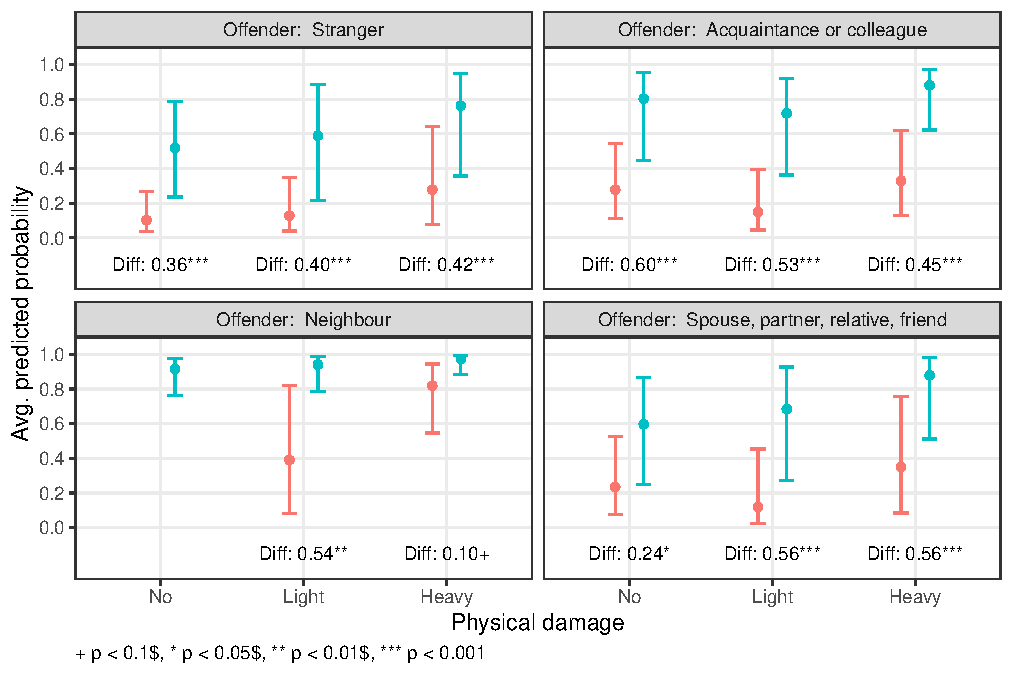
\includegraphics[width = \textwidth]{figures/avg_predicted_probs_grouped.pdf}
 	\caption{Predictions from model}
 	\label{fig:predictions}	
\end{figure}

\subsection{Robustness checks}
\label{subsec:robust}

Addressing possible
\begin{enumerate}
    \item endogeneity:
    \begin{itemize}
        \item failed IV (only a mention, regression result not included)
        \item subset of crime with close offenders
    \end{itemize}
    \item ommitted variables: emotional damage, trust in police
    \begin{itemize}
        \item regression on 2024 data with inclusion ommitted vars
    \end{itemize}
\end{enumerate}

\begin{table}
	\caption{Logistic regression result after controlling for police trust and emotional damage, 2024 data only}
	\label{table:regr_2024}
	\begin{adjustbox}{width=1\textwidth}
		\begin{tabular}{lccccc}
\toprule
  & Theft & Cybercrime & All property & Assault & All violent \\ 
\midrule\addlinespace[2.5pt]
Told someone & 0.045 & 0.539+ & 0.486 & 2.569** & 2.510** \\ 
Financial: (1, 10] thnd rub. & -0.039 & 0.700 & 0.397 & 0.910 & 0.752 \\ 
Financial: (10, 50] thnd rub. & 0.871+ & 1.209** & 0.990** & 0.298 & 0.749 \\ 
Financial: (50, Inf] thnd rub. & 1.363** & 2.193*** & 1.770*** & 0.786 & 0.972+ \\ 
Physical: Light &  &  &  & -0.142 & -0.104 \\ 
Physical: Heavy &  &  &  & 0.934 & 0.905 \\ 
Emotional: Medium & 0.870+ & 0.072 & 0.247 & -1.084 & -0.982 \\ 
Emotional: Heavy & 1.252* & 0.816* & 0.893** & -0.207 & 0.052 \\ 
Incident: Witness &  &  &  & 0.747 & 0.645+ \\ 
Incident: Victim resisted &  &  &  & -0.531 & -0.918* \\ 
Incident: Weapon &  &  &  & 0.673 & 0.431 \\ 
Self-blame & -0.395 & -0.399 & -0.477* & -0.405 & -0.532 \\ 
Has partner & -0.089 & -0.073 & -0.055 & 0.073 & 0.125 \\ 
Off. rel.: Acquaintance or colleague &  &  &  & 1.612* & 1.575* \\ 
Off. rel.: Neighbour &  &  &  & 1.956* & 1.919** \\ 
Off. rel.: Spouse, partner, relative, friend &  &  &  & 0.321 & 0.546 \\ 
Gender: Male & 0.084 & 0.137 & 0.080 & -0.412 & -0.332 \\ 
Income: Can buy furniture/electonics & -0.115 & 0.073 & 0.005 & 0.733 & 0.708+ \\ 
Income: Can buy a car, or higher & -0.526 & -0.311 & -0.452 & -0.139 & -0.143 \\ 
Highly educated & 0.810* & 0.333* & 0.389** & 0.061 & -0.008 \\ 
Settlement: Small town & 0.236 & -0.289 & -0.161 & 0.586 & 0.415 \\ 
Settlement: Village & -0.159 & -0.096 & -0.250 & 0.556 & 0.258 \\ 
Settlement: Unknown & 1.628 & -0.697 & 0.088 & 0.555 & 0.415 \\ 
Attitude: Victim trusts the police & 0.307 & 0.336 & 0.310 & -0.065 & 0.127 \\ 
Attitude: Victim knows a police & -0.212 & -0.195 & -0.180 & 0.270 & 0.429 \\ 
{Attitude: Victim has crime record} & {0.339} & {0.077} & {0.247} & {0.494} & {0.536} \\ 
\midrule
Num.Obs. & 405 & 703 & 1143 & 260 & 304 \\ 
R2 & 0.094 & 0.076 & 0.058 & 0.251 & 0.254 \\ 
R2 Adj. & -0.030 & 0.005 & 0.015 & 0.010 & 0.045 \\ 
R2 Within & 0.135 & 0.136 & 0.120 & 0.264 & 0.272 \\ 
R2 Within Adj. & 0.052 & 0.090 & 0.092 & 0.086 & 0.117 \\ 
RMSE & 0.44 & 0.45 & 0.45 & 0.41 & 0.41 \\ 
Std.Errors clustered by federal district& X & X & X & X & X \\ 
FE: federal\_district & X & X & X & X & X \\ 
\bottomrule
\multicolumn{6}{l}{\small + p < 0.1, * p < 0.05, ** p < 0.01, *** p < 0.001}\\
\end{tabular}

	\end{adjustbox}
\end{table}



\section{Discussion}
\label{sec:discussion}
Scarcity of research on connection between seeking informal help and reporting may in part be due to there are seemingly no immediate policy implications \citep{greenberg1992after}. However, 1) it may be more effective to work through situational advisors (victim decision making being compromised by shock), i.e. potentially anyone; 2) if we believe that consulting others heightens probability of reporting we must conclude that lonely people report less, which gives us an insight on the direction of bias introduced by under-reporting crime.

\section{Conclusion}
\label{sec:conclusion}

\bibliographystyle{apacite}
\bibliography{bib.bib}

%
%\section{Appendices}
%
%Any appendices should be placed after the list of references, beginning with the command \verb"\appendix" followed by the command \verb"\section" for each appendix title, e.g.
%\begin{verbatim}
%\appendix
%\section{This is the title of the first appendix}
%\section{This is the title of the second appendix}
%\end{verbatim}
%produces:\medskip
%
%\noindent\textbf{Appendix A. This is the title of the first appendix}\medskip
%
%\noindent\textbf{Appendix B. This is the title of the second appendix}\medskip
%
%\noindent Subsections, equations, figures, tables, etc.\ within appendices will then be automatically numbered as appropriate. Some theorem-like environments may need to have their counters reset manually (e.g.\ if they are not numbered within sections in the main text). You can achieve this by using \verb"\numberwithin{remark}{section}" (for example) just after the \verb"\appendix" command.
%
%Note that if the \verb"endfloat" package is used on a document containing any appendices, the \verb"\processdelayedfloats" command must be included immediately before the \verb"\appendix" command in order to ensure that the floats belonging to the main body of the text are numbered as such.
%
%%\processdelayedfloats %%% See above for an explanation of why this command might be needed here.
%
%\appendix
%
%\section{Troubleshooting}
%
%Authors may occasionally encounter problems with the preparation of a manuscript using \LaTeX. The appropriate action to take will depend on the nature of the problem:
%\begin{enumerate}
%\item[(i)] If the problem is with \LaTeX\ itself, rather than with the actual macros, please consult an appropriate \LaTeXe\ manual for initial advice. If the solution cannot be found, or if you suspect that the problem does lie with the macros, then please contact Taylor \& Francis for assistance (\texttt{latex.helpdesk@tandf.co.uk}), clearly stating the title of the journal to which you are submitting.
%\item[(ii)] Problems with page make-up (e.g.\ occasional overlong lines of text; figures or tables appearing out of order): please do not try to fix these using `hard' page make-up commands -- the typesetter will deal with such problems. (You may, if you wish, draw attention to particular problems when submitting the final version of your manuscript.)
%\item[(iii)] If a required font is not available on your system, allow \TeX\ to substitute the font and specify which font is required in a covering letter accompanying your files.
%\end{enumerate}
%
%
%\section{Obtaining the template and class file}
%
%\subsection{Via the Taylor \& Francis website}
%
%This article template and the \texttt{interact} class file may be obtained via the `Instructions for Authors' pages of selected Taylor \& Francis journals.
%
%Please note that the class file calls up the open-source \LaTeX\ packages booktabs.sty, epsfig.sty and rotating.sty, which will, for convenience, unpack with the downloaded template and class file. The template optionally calls for natbib.sty and subfig.sty, which are also supplied for convenience.
%
%
%\subsection{Via e-mail}
%
%This article template, the \texttt{interact} class file and the associated open-source \LaTeX\ packages are also available via e-mail. Requests should be addressed to \texttt{latex.helpdesk@tandf.co.uk}, clearly stating for which journal you require the template and class file.

\end{document}
